\documentclass[a4paper,11pt]{article}
\usepackage[utf8]{inputenc}
% \usepackage[normalem]{ulem}

% \usepackage{amssymb}
\usepackage{amsmath,color,amssymb,graphicx}
\definecolor{navy}{rgb}{0,0.2,0.7}
\usepackage{pxfonts}
\usepackage[pdftex,
           hyperindex=true,
           colorlinks=true,
           linkcolor=navy,
           anchorcolor=magenta,
           citecolor=navy,
           urlcolor=navy,
           unicode,
           implicit=true]{hyperref}
\renewcommand{\vec}[1]{\boldsymbol{#1}}           
\usepackage[paperwidth=21.0cm,paperheight=29.7cm,textwidth=16cm,textheight=20cm,top=2cm,left=3.cm,bottom=2cm]{geometry}
\usepackage[backend=biber,firstinits=true,isbn=false,url=false,dashed=false,style=authoryear,maxcitenames=1,maxbibnames=99]{biblatex}
\renewbibmacro{in:}{}
\addbibresource{references_project.bib}

%opening
\title{Effect of the icebergs' capsize on the glacier motion}
\author{V.A. Yastrebov}


\begin{document}

\maketitle


\section{Single iceberg-capsize scenario}

\begin{figure}[htb!]
 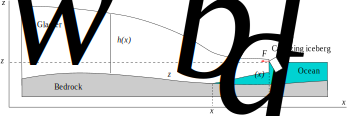
\includegraphics[width=1\textwidth]{setup_glacier}
 \caption{\label{fig:1}Marine-terminating glacier}
\end{figure}

We consider the effect of a single iceberg capsize on the deformation of the glacier for various simple models of a bedrock and different glacier tongues.
We assume that the terminus is located at $x=L$ for the glacier sliding from left to right, i.e. from smaller to greater values of $x$.
The following bedrock models $z_b$ (lower script $b$ stands for basal) near the terminus are considered:
\begin{enumerate}
 \item Flat bedrock $z_b(x)  = z_0$ 
 \item Linear positive slope $z_b(x) = z_0 - a x$, $a>0$
 \item Linear negative slope $z_b(x) = z_0 + a x$, $a>0$
 \item Parabolic positive slope $z_b(x) = z_0 - b x^2$, $b>0$
 \item Parabolic negative slope $z_b(x) = z_0 + b x^2$, $b>0$
 \item Wavy slope $z_b(x) = z_0 + c \sin(2\pi (x + s)/\lambda)$, where the shift $s \in (0,\lambda)$
 \item Random self-affine bedrock $z_b = z_b(x,H,\langle z \rangle, \langle \nabla z \rangle, \langle (z - \langle z\rangle)^2 \rangle)$, where $H \in (0,1)$ is the Hurst exponent, $\langle \bullet \rangle$ denotes the mean value.
\end{enumerate}
In addition, we will consider glaciers with and without tongue
\begin{enumerate}
 \item Glacier without tongue, positive effective basal pressure $p(L) - \rho_w g h(L) \ge 0$, where $h(x)$ is the iceberg's height 
 \item Glacier with a tongue, negative effective pressure at terminus $p(L) - \rho_w gh(L) < 0$, for various lengths of the glacier tongue $L-x_g$, where the grounding point $x_g:\; p(x_g) = \rho_w g h$
\end{enumerate}
And finally, we will consider various friction laws listed below:
\begin{enumerate}
 \item Weertman friction
 \item Coulomb friction
 \item Schoof friction
\end{enumerate}
For every initial configuration, the aspect ratio of the iceberg has to be selected such that it produces the maximal pic force on the glacier; the height of the iceberg will be unambiguously determined by the ice thickness at the terminus. 
The water level should be meaningful, i.e. near the hydrostatic equilibrium $h(x_g) - z_w \pm \Delta z_w + z_b(x_g) = \rho_i h(x_g) / \rho_w $, i.e. 
\[z_w = h(x_g) + z_b(x_g) - \rho_i h(x_g) / \rho_w \pm \Delta z_w.\]
The spatial discretization $\Delta x$ should such that \[ \forall x: \; z_b(x+\Delta x) - z_b(x) \ll \Delta x\].
The interest of this study is two-fold: 
\begin{itemize}
 \item[(1)] construct parametric maps to determine parameters resulting in reverse motion of the glacier;
 \item[(2)] investigate possible seismicity related to the motion of the glacier.
\end{itemize}

However the ice thickness $h(x)$ for the considered bedrock models cannot be selected arbitrary. The evolution of iceberg thickness should follow the equations derived in~\parencite{muszynski1987coupled,schoof2007marine,tsai2015marine}.

\section{Multiple iceberg-capsize scenario}

Starting from a feasible configuration for the marine-terminating glacier, we will simulate a sequence of iceberg calving with a certain probability density of temporal and spatial distributions for iceberg aspect ratio and time periods between different calving events. For example, the following sequences could be generated for a given scenario, the time of calving events:
\[
 \vec T = \{0, 1\,200, 56\,000, 121\,000, \dots \} \text{ [s]}
\]
and the corresponding aspect ratios:
\[
 \vec \epsilon = \{0.30, 0.43, 1.2, 0.22 \dots \} \text{ [-]}
\]
Of course, at such long time periods the equation of glacier flow should be accounted for.



\printbibliography[heading=bibintoc]




\end{document}
